\documentclass[12pt, titlepage]{article}

\usepackage{fullpage}
\usepackage[round]{natbib}
\usepackage{multirow}
\usepackage{booktabs}
\usepackage{tabularx}
\usepackage{graphicx}
\usepackage{float}
\usepackage{hyperref}
\hypersetup{
    colorlinks,
    citecolor=black,
    filecolor=black,
    linkcolor=red,
    urlcolor=blue
}
\usepackage[round]{natbib}

\newcounter{acnum}
\newcommand{\actheacnum}{AC\theacnum}
\newcommand{\acref}[1]{AC\ref{#1}}

\newcounter{ucnum}
\newcommand{\uctheucnum}{UC\theucnum}
\newcommand{\uref}[1]{UC\ref{#1}}

\newcounter{mnum}
\newcommand{\mthemnum}{M\themnum}
\newcommand{\mref}[1]{M\ref{#1}}

\title{SE 3XA3: Module Guild\\\textbf{Snake Game Remake}}

\author{Team \#, 302, Team Name: 404
		\\ Student: Shunbo Cui	    cuis13
		\\ Student: Xiangxin Kong	kongx9
		\\ Student: Shuo Zhang	    zhans18
}
\date{March 13, 2020}

\begin{document}

\maketitle

\pagenumbering{roman}
\tableofcontents
\listoftables
\listoffigures

\begin{table}[H]
\caption{\bf Revision History}
\begin{tabularx}{\textwidth}{p{3cm}p{2cm}X}
\toprule {\bf Date} & {\bf Version} & {\bf Notes}\\
\midrule
March 13, 2020 & Shuo Zhang, Xiangxin Kong, Shunbo Cui & Create the MG\\
April 6, 2020 & Shuo Zhang, Xiangxin Kong, Shunbo Cui & Edit Part 5,6,7\\
\bottomrule
\end{tabularx}
\end{table}

\newpage

\pagenumbering{arabic}

\section{Introduction}

\subsection{Overview} \label{SecAchange}

Snake-Game-remake is a Java game developed for providing an enjoyable and challenging 
gaming experience for the user. It is a game inspired by Snake-Java-2D-game which 
focuses on the growth of a snake character by consuming the food items generated
in the game map. The snake keeps moving and the player can adjust the direction
to the left or right. The player has to navigate the snake to avoid collision 
with the boarder of the map and other barriers, as well as its own body. The team's
main purpose of the project is to modularize the structure so that it will be easier 
to add more functions and features to the system. The Module Interface Specification 
is created, which explains the breakdown of the project for each module.

\subsection{Scope} \label{SecAchange}

The scope of this project is to implement the 2D Java game board and additional functions.
 The team is going to add more functions such as leader board, restart option and more in-game 
 items. The user interface is also going to be reconstructed. All the additional function will 
 be implemented in individual Java modules with high cohesion.
\subsection{Document structure} \label{SecAchange}
The rest of the document is organized as follows. 
\begin{itemize}
    \item Section\ref{SecChange} lists the anticipated and unlikely changes of the software
requirements.
    \item Section \ref{SecMH} summarizes the module decomposition that
was constructed according to the likely changes. 
    \item Section \ref{SecConnection}
specifies the connections between the software requirements and the
modules. 
    \item Section \ref{SecMD} gives a detailed description of the
modules. 
    \item Section \ref{SecTM} includes two traceability matrices. One checks
the completeness of the design against the requirements provided in the SRS. The
other shows the relation between anticipated changes and the modules. 
    \item Section \ref{SecUse} describes the use relation between modules.
\end{itemize} 


\section{Anticipated and Unlikely Changes} \label{SecChange}

This section lists possible changes our team considering to make. According to the likeliness
of the change, the possible changes are classified into two
categories. Anticipated changes are listed in Section \ref{SecAchange}, and
unlikely changes are listed in Section \ref{SecUchange}.

\subsection{Anticipated Changes} \label{SecAchange}

Anticipated changes are the source of the information that is to be hidden
inside the modules. Ideally, changing one of the anticipated changes will only
require changing the one module that hides the associated decision. The approach
adapted here is called design for
change.

\begin{description}
\item[\refstepcounter{acnum} \actheacnum \label{acInput}:] The format of the input data.
\item[\refstepcounter{acnum} \actheacnum \label{acSettings}:] Default player settings for input.
\item[\refstepcounter{acnum} \actheacnum \label{acHardware}:] The hardware on which the software is ran.
\item[\refstepcounter{acnum} \actheacnum \label{acTextures}:] The in-game textures of snake, map and items.
\end{description}

\subsection{Unlikely Changes} \label{SecUchange}

The module design should be as general as possible. However, a general system is
more complex. Sometimes this complexity is not necessary. Fixing some design
decisions at the system architecture stage can simplify the software design. If
these decision should later need to be changed, then many parts of the design
will potentially need to be modified. Hence, it is not intended that these
decisions will be changed.

\begin{description}
\item[\refstepcounter{ucnum} \uctheucnum \label{ucIO}:] Input/Output devices
  (Input: Keyboard, Output: Speaker, Screen). Keyboard is essential to enable the function of 
  multiplayer in the same game. The speaker is used to play effect sound in the game and screen 
  for displaying.
\item[\refstepcounter{ucnum} \uctheucnum \label{ucMap}:] The method of defining a map. A lot of 
other components in the system requires to be changed if this part of design is modified.
\end{description}

\section{Module Hierarchy} \label{SecMH}

This section provides an overview of the module design. Modules are summarized
in a hierarchy decomposed by secrets in Table \ref{TblMH}. The modules listed
below, which are leaves in the hierarchy tree, are the modules that will
actually be implemented.

\begin{description}
\item [\refstepcounter{mnum} \mthemnum \label{mHardwareHiding}:] Main module
\item [\refstepcounter{mnum} \mthemnum \label{mGamePanel}:] Game panel
\item [\refstepcounter{mnum} \mthemnum \label{mSnake}:] Snake
\item [\refstepcounter{mnum} \mthemnum \label{mFoodItem}:] Food and Item
\item [\refstepcounter{mnum} \mthemnum \label{mMap}:] Map
\item [\refstepcounter{mnum} \mthemnum \label{mSoundEffect}:] Sound effect
\item [\refstepcounter{mnum} \mthemnum \label{mMain}:] Main
\item [\refstepcounter{mnum} \mthemnum \label{mColor}:] Color
\item [\refstepcounter{mnum} \mthemnum \label{mInput}:] Input Manager
\end{description}


\begin{table}[h!]
\centering
\begin{tabular}{p{0.3\textwidth} p{0.6\textwidth}}
\toprule
\textbf{Level 1} & \textbf{Level 2}\\
\midrule

{Hardware-Hiding Module} &  \\
\midrule

\multirow{3}{0.3\textwidth}{Behaviour-Hiding Module} & Map\\
~ & Sound Effect\\
~ & Game Panel\\
~ & Main\\
~ & Color\\
~ & InputManager\\
\midrule

\multirow{2}{0.3\textwidth}{Software Decision Module} & Snake\\
~ & Food and Item\\
\bottomrule

\end{tabular}
\caption{Module Hierarchy}
\label{TblMH}
\end{table}

\section{Connection Between Requirements and Design} \label{SecConnection}

The design of the system is intended to satisfy the requirements developed in
the SRS. In this stage, the system is decomposed into modules. The connection
between requirements and modules is listed in Table \ref{TblRT}.

\section{Module Decomposition} \label{SecMD}

Modules are decomposed according to the principle of ``information hiding''
proposed by \citet{ParnasEtAl1984}. The \emph{Secrets} field in a module
decomposition is a brief statement of the design decision hidden by the
module. The \emph{Services} field specifies \emph{what} the module will do
without documenting \emph{how} to do it. For each module, a suggestion for the
implementing software is given under the \emph{Implemented By} title. If the
entry is \emph{OS}, this means that the module is provided by the operating
system or by standard programming language libraries.  Also indicate if the
module will be implemented specifically for the software.

Only the leaf modules in the
hierarchy have to be implemented. If a dash (\emph{--}) is shown, this means
that the module is not a leaf and will not have to be implemented. Whether or
not this module is implemented depends on the programming language
selected.

\subsection{Hardware Hiding Modules (\mref{mHardwareHiding})}

\begin{description}
\item[Secrets:]The data structure and algorithm used to implement the virtual input and 
output hardware such as keyboard and the screen.
\item[Services:]Serves as a virtual hardware used by the rest of the
  system. This module provides the interface between the hardware and the
  software. So, the system can use it to display outputs or to accept inputs.
\item[Implemented By:] OS and Java Virtual Machine
\end{description}

\subsection{Behaviour-Hiding Module}

\begin{description}
\item[Secrets:]The contents of the required behaviours.
\item[Services:]Includes programs that provide externally visible behaviour of
  the system as specified in the software requirements specification (SRS)
  documents. This module serves as a communication layer between the
  hardware-hiding module and the software decision module. The programs in this
  module will need to change if there are changes in the SRS.
\end{description}

\subsubsection{Game panel module (\mref{mGamePanel})}

\begin{description}
\item[Secrets:]The game panel generation and interaction.
\item[Services:]Construct the basic panel as the game board.
\item[Implemented By:] Java Libraries
\end{description}

\subsubsection{Game map construction module (\mref{mMap})}

\begin{description}
\item[Secrets:]The game map constructions.
\item[Services:]Construct the game map from the input data from the map files.
\item[Implemented By:] Java Libraries
\end{description}

\subsubsection{Sound effect control module (\mref{mSoundEffect})}

\begin{description}
\item[Secrets:]The sound effect controls.
\item[Services:]Details the sound effect used in the game.
\item[Implemented By:] Java Libraries
\end{description}

\subsubsection{Main module (\mref{mMain})}

\begin{description}
\item[Secrets:]The choices from Users.
\item[Services:]Construct panel for user to make game choices and setting before game start.
\item[Implemented By:] Java Libraries
\end{description}

\subsubsection{Color module (\mref{mColor})}

\begin{description}
\item[Secrets:]The color controls.
\item[Services:]Details the color used in the game.
\item[Implemented By:] Java Libraries
\end{description}

\subsubsection{Input manager module (\mref{mInput})}

\begin{description}
\item[Secrets:]The Input key controls.
\item[Services:]Details the keyboard keys used in the game.
\item[Implemented By:] Java Libraries
\end{description}

\subsection{Software Decision Module}

\begin{description}
\item[Secrets:] The design decision based on mathematical theorems, physical
  facts, or programming considerations. The secrets of this module are
  \emph{not} described in the SRS.
\item[Services:] Includes data structure and algorithms used in the system that
  do not provide direct interaction with the user. 
  % Changes in these modules are more likely to be motivated by a desire to
  % improve performance than by externally imposed changes.
\item[Implemented By:] --
\end{description}

\subsubsection{Snake module (\mref{mSnake})}

\begin{description}
\item[Secrets:]Algorithms implemented for generation and interaction of snakes in the game.
\item[Services:]Provides the data structure and algorithms for generation and interaction of snakes in the game.
\item[Implemented By:] Java Libraries
\end{description}

\subsubsection{Food and Item module (\mref{mFoodItem})}

\begin{description}
\item[Secrets:]Algorithms implemented for generation and interaction of all in-game items.
\item[Services:]Provides the data structure and algorithms for generation and interaction of in-game items.
\item[Implemented By:] Java Libraries
\end{description}

\section{Traceability Matrix} \label{SecTM}

This section shows two traceability matrices: between the modules and the
requirements and between the modules and the anticipated changes.

% the table should use mref, the requirements should be named, use something




% like fref
\begin{table}[H]
\centering
\begin{tabular}{p{0.2\textwidth} p{0.6\textwidth}}
\toprule
\textbf{Req.} & \textbf{Modules}\\
\midrule
FR1 & \mref{mHardwareHiding}, \mref{mGamePanel}, \mref{mSnake}, \mref{mFoodItem}, \mref{mMap}, \mref{mSoundEffect}, \mref{mMain}, \mref{mColor}, \mref{mInput}\\
FR2 & \mref{mGamePanel}, \mref{mMain}\\
FR3 & \mref{mGamePanel}, \mref{mMain}\\
FR4 & \mref{mGamePanel}, \mref{mMap}, \mref{mMain}\\
FR5 & \mref{mGamePanel}, \mref{mMap}, \mref{mColor}\\
FR6 & \mref{mGamePanel}, \mref{mSnake}, \mref{mMap}\\
FR7 & \mref{mGamePanel}, \mref{mSnake}\\
FR8 & \mref{mGamePanel}, \mref{mFoodItem}, \mref{mMap}\\
FR9 & \mref{mGamePanel}\\
FR10 & \mref{mGamePanel}\\
FR11 & \mref{mGamePanel}\\
FR12 & \mref{mGamePanel}, \mref{mSnake}, \mref{mFoodItem}, \mref{mSoundEffect}\\
FR13 & \mref{mGamePanel}, \mref{mMap}, \mref{mFoodItem}\\
FR14 & \mref{mGamePanel}, \mref{mSnake}\\
FR15 & \mref{mGamePanel}, \mref{mFoodItem}, \mref{mMap}\\
FR16 & \mref{mGamePanel}, \mref{mFoodItem}, \mref{mMap}, \mref{mSnake}, \mref{mSoundEffect}\\
FR17 & \mref{mGamePanel}, \mref{mSnake}, \mref{mMap}, \mref{mSoundEffect}\\
FR18 & \mref{mGamePanel}\\
FR19 & \mref{mGamePanel}, \mref{mColor}, \mref{mMain}\\
FR20 & \mref{mGamePanel}, \mref{mInput}\\
\bottomrule
\end{tabular}
\caption{Trace Between Requirements and Modules}
\label{TblRT}
\end{table}

\begin{table}[H]
\centering
\begin{tabular}{p{0.2\textwidth} p{0.6\textwidth}}
\toprule
\textbf{AC} & \textbf{Modules}\\
\midrule
\acref{acInput} & \mref{mGamePanel}\\
\acref{acSettings} & \mref{mGamePanel}\\
\acref{acHardware} & \mref{mHardwareHiding}\\
\acref{acTextures} & \mref{mGamePanel}\\
\bottomrule
\end{tabular}
\caption{Trace Between Anticipated Changes and Modules}
\label{TblACT}
\end{table}

\section{Use Hierarchy Between Modules} \label{SecUse}

In this section, the uses hierarchy between modules is
provided. \citet{Parnas1978} said of two programs A and B that A {\em uses} B if
correct execution of B may be necessary for A to complete the task described in
its specification. That is, A {\em uses} B if there exist situations in which
the correct functioning of A depends upon the availability of a correct
implementation of B.  Figure \ref{FigUH} illustrates the use relation between
the modules. It can be seen that the graph is a directed acyclic graph
(DAG). Each level of the hierarchy offers a testable and usable subset of the
system, and modules in the higher level of the hierarchy are essentially simpler
because they use modules from the lower levels.

\begin{figure}[H]
\centering
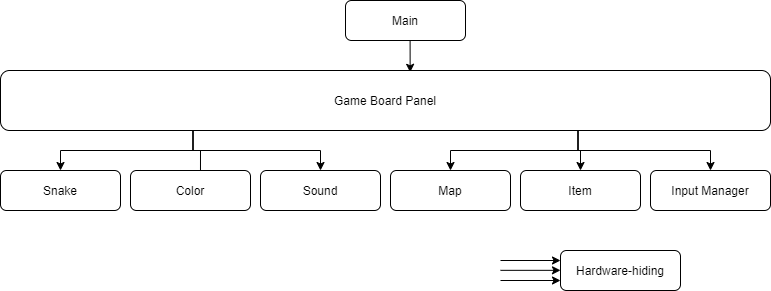
\includegraphics[width=0.7\textwidth]{UsesHierarchy.png}
\caption{Use hierarchy among modules}
\label{FigUH}
\end{figure}

%\section*{References}

\bibliographystyle {plainnat}
\bibliography {MG}

\end{document}
